% Topic T5.1: What Goes Wrong
% Self-contained Beamer slides for Digital Finance course
\documentclass[11pt,aspectratio=169]{beamer}
\usetheme{Madrid}

% ======================= PACKAGES =======================
\usepackage{graphicx}
\usepackage{booktabs}
\usepackage{adjustbox}
\usepackage{multicol}
\usepackage{amsmath}
\usepackage{amssymb}
\usepackage{tikz}
\usetikzlibrary{arrows,shapes,positioning,shadows,trees}
\usepackage{listings}
\usepackage{xcolor}

% ======================= COLOR DEFINITIONS =======================
% Primary color scheme: Blue/Teal for Digital Finance
\definecolor{dfblue}{RGB}{0,102,204}
\definecolor{dfteal}{RGB}{0,153,153}
\definecolor{dfcyan}{RGB}{51,187,204}
\definecolor{dflightblue}{RGB}{153,204,255}
\definecolor{dflightblue2}{RGB}{173,214,255}
\definecolor{dflightblue3}{RGB}{193,224,255}
\definecolor{dflightblue4}{RGB}{213,234,255}

% Accent colors for finance applications
\definecolor{dfgreen}{RGB}{44, 160, 44}
\definecolor{dfred}{RGB}{214, 39, 40}
\definecolor{dforange}{RGB}{255, 127, 14}
\definecolor{dfgray}{RGB}{127, 127, 127}

% Utility colors
\definecolor{lightgray}{RGB}{240, 240, 240}
\definecolor{midgray}{RGB}{180, 180, 180}
\definecolor{codebg}{RGB}{245, 245, 245}

% ======================= THEME CUSTOMIZATION =======================
% Apply Digital Finance color scheme to Madrid theme
\setbeamercolor{palette primary}{bg=dflightblue3,fg=dfblue}
\setbeamercolor{palette secondary}{bg=dflightblue2,fg=dfblue}
\setbeamercolor{palette tertiary}{bg=dfteal,fg=white}
\setbeamercolor{palette quaternary}{bg=dfblue,fg=white}

\setbeamercolor{structure}{fg=dfblue}
\setbeamercolor{section in toc}{fg=dfblue}
\setbeamercolor{subsection in toc}{fg=dfteal}
\setbeamercolor{title}{fg=dfblue}
\setbeamercolor{frametitle}{fg=dfblue,bg=dflightblue3}
\setbeamercolor{block title}{bg=dflightblue2,fg=dfblue}
\setbeamercolor{block body}{bg=dflightblue4,fg=black}

% Remove navigation symbols for cleaner look
\setbeamertemplate{navigation symbols}{}

% Clean itemize/enumerate
\setbeamertemplate{itemize items}[circle]
\setbeamertemplate{enumerate items}[default]

% Margins for readability
\setbeamersize{text margin left=8mm,text margin right=8mm}

% ======================= LISTINGS CONFIGURATION =======================
% Python code style
\lstdefinestyle{pythonstyle}{
    language=Python,
    basicstyle=\ttfamily\footnotesize,
    keywordstyle=\color{dfblue}\bfseries,
    stringstyle=\color{dforange},
    commentstyle=\color{dfgray}\itshape,
    numberstyle=\tiny\color{dfgray},
    numbers=left,
    numbersep=5pt,
    backgroundcolor=\color{codebg},
    showspaces=false,
    showstringspaces=false,
    showtabs=false,
    frame=single,
    rulecolor=\color{midgray},
    tabsize=4,
    captionpos=b,
    breaklines=true,
    breakatwhitespace=false,
    escapeinside={(*@}{@*)},
    xleftmargin=10pt,
    xrightmargin=10pt
}

% Solidity code style
\lstdefinestyle{soliditystyle}{
    language=Java, % closest approximation
    basicstyle=\ttfamily\footnotesize,
    keywordstyle=\color{dfteal}\bfseries,
    stringstyle=\color{dforange},
    commentstyle=\color{dfgray}\itshape,
    numberstyle=\tiny\color{dfgray},
    numbers=left,
    numbersep=5pt,
    backgroundcolor=\color{codebg},
    showspaces=false,
    showstringspaces=false,
    showtabs=false,
    frame=single,
    rulecolor=\color{midgray},
    tabsize=2,
    captionpos=b,
    breaklines=true,
    breakatwhitespace=false,
    escapeinside={(*@}{@*)},
    xleftmargin=10pt,
    xrightmargin=10pt,
    morekeywords={pragma, contract, function, returns, public, private, view, pure, payable, address, uint256, mapping, event, modifier}
}

% Inline code command
\newcommand{\code}[1]{\texttt{\color{dfblue}#1}}

% ======================= CUSTOM COMMANDS =======================
% Bottom annotation (Madrid-style)
\newcommand{\bottomnote}[1]{%
\vfill
\vspace{-2mm}
\textcolor{dflightblue2}{\rule{\textwidth}{0.4pt}}
\vspace{1mm}
\footnotesize
\textbf{#1}
}

% Compact list spacing
\newcommand{\compactlist}{%
\setlength{\itemsep}{0pt}%
\setlength{\parskip}{0pt}%
\setlength{\parsep}{0pt}%
}

% Chart placeholder
\newcommand{\chartplaceholder}[2][5cm]{%
\begin{center}
\begin{adjustbox}{max width=0.95\textwidth, max height=#1}
\framebox[\textwidth][c]{%
\rule{0pt}{#1}%
\textcolor{midgray}{[#2]}%
}
\end{adjustbox}
\end{center}
}

% ======================= FINANCE NOTATION MACROS =======================
% Probability and statistics
\newcommand{\E}{\mathbb{E}} % Expected value
\newcommand{\Var}{\mathrm{Var}} % Variance
\newcommand{\Cov}{\mathrm{Cov}} % Covariance
\newcommand{\Prob}{\mathbb{P}} % Probability

% Distributions
\newcommand{\Normal}{\mathcal{N}} % Normal distribution
\newcommand{\Uniform}{\mathcal{U}} % Uniform distribution

% Returns and prices
\newcommand{\Ret}{R} % Return
\newcommand{\LogRet}{r} % Log return
\newcommand{\Price}{S} % Price/Stock price
\newcommand{\Strike}{K} % Strike price

% Options and derivatives
\newcommand{\CallPrice}{C} % Call option price
\newcommand{\PutPrice}{P} % Put option price
\newcommand{\Greeks}[1]{\mathit{#1}} % Greek letters

% Risk measures
\newcommand{\VaR}{\mathrm{VaR}} % Value at Risk
\newcommand{\CVaR}{\mathrm{CVaR}} % Conditional VaR
\newcommand{\Sharpe}{\mathrm{SR}} % Sharpe Ratio

% Time series
\newcommand{\AR}{\mathrm{AR}} % Autoregressive
\newcommand{\MA}{\mathrm{MA}} % Moving average
\newcommand{\GARCH}{\mathrm{GARCH}} % GARCH

% Blockchain/Crypto
\newcommand{\Hash}{\mathrm{Hash}} % Hash function
\newcommand{\Block}{\mathcal{B}} % Block
\newcommand{\Chain}{\mathcal{C}} % Chain

% Real numbers, integers
\newcommand{\R}{\mathbb{R}}
\newcommand{\Z}{\mathbb{Z}}
\newcommand{\N}{\mathbb{N}}

% ======================= TIKZ STYLES =======================
% Styles for finance-related diagrams
\tikzstyle{process} = [rectangle, minimum width=3cm, minimum height=1cm, text centered, draw=dfblue, fill=dflightblue4, thick]
\tikzstyle{decision} = [diamond, minimum width=3cm, minimum height=1cm, text centered, draw=dfteal, fill=dflightblue4, thick]
\tikzstyle{arrow} = [thick,->,>=stealth,color=dfblue]
\tikzstyle{blockchain} = [rectangle, rounded corners, minimum width=2.5cm, minimum height=1cm, text centered, draw=dfteal, fill=dflightblue3, thick]
\tikzstyle{transaction} = [circle, minimum size=0.8cm, text centered, draw=dforange, fill=dflightblue4, thick]

% ======================= FOOTER TEMPLATE =======================
\setbeamertemplate{footline}{
    \hbox{\begin{beamercolorbox}[wd=\paperwidth,ht=2.5ex,dp=1ex,leftskip=.5em,rightskip=.5em]{author in head/foot}
    \tiny
    \textbf{Digital Finance} \hfill
    Joerg Osterrieder \hfill
    \insertdate \hfill
    Page \insertframenumber{} / \inserttotalframenumber
    \end{beamercolorbox}}
}

% ======================= SECTION DIVIDER TEMPLATE =======================
\AtBeginSection[]{
\begin{frame}[plain]
\vfill
\centering
\begin{beamercolorbox}[sep=12pt,center]{title}
\usebeamerfont{title}\LARGE\insertsection\par
\end{beamercolorbox}
\vfill
\end{frame}
}


\title[T5.1: What Goes Wrong]{Topic 5.1: What Goes Wrong}
\subtitle{Failures, Hacks, and Systemic Risk in Digital Finance}
\author{Joerg Osterrieder}
\institute{Digital Finance}
\date{2025}

\begin{document}

% =============================================================================
% Frame 1: Title Slide
% =============================================================================
\begin{frame}[plain]
\titlepage
\end{frame}

% =============================================================================
% Frame 2: Learning Objectives
% =============================================================================
\begin{frame}{Learning Objectives}
\begin{center}
\textbf{\Large What You Will Learn in This Topic}
\end{center}

\vspace{5mm}
By the end of this session, you will be able to:

\begin{enumerate}
%% H14: Simplified learning objectives -- removed jargon like "reentrancy, flash loans, oracle manipulation"
\item \textbf{Categorize} types of digital finance failures (technical, economic, human)
\item \textbf{Explain} how the major types of attacks work, using plain-English descriptions and analogies
\item \textbf{Analyze} case studies of historical DeFi hacks
\item \textbf{Assess} how the interconnection of protocols creates cascading risk
\item \textbf{Develop} genuine risk awareness for evaluating digital finance systems
\end{enumerate}

\vspace{5mm}
\begin{block}{Hands-On Component}
Colab notebook (NB11) simulating historical DeFi exploits---run reentrancy, flash loan, and oracle manipulation scenarios to understand how attacks work.
\end{block}
\end{frame}

% =============================================================================
% Frame 3: Prerequisites/Background I
% =============================================================================
%% C1: Removed "Basic Solidity syntax" prerequisite; replaced with accessibility note
%% C5: Day 4-to-Day 5 transition content integrated into this frame
\begin{frame}{Prerequisites: What You Should Know}
\begin{columns}[T]
\begin{column}{0.48\textwidth}
\textbf{Required Background:}
\begin{itemize}
\item Basic understanding of smart contracts
\item Familiarity with DeFi concepts (lending, DEXs)
\item Understanding of blockchain transactions
\end{itemize}

\vspace{3mm}
\textbf{Helpful but not required:}
\begin{itemize}
\item No coding knowledge needed---all technical concepts explained visually
\item Knowledge of token standards (ERC-20)
\item Experience with DeFi protocols
\end{itemize}
\end{column}
\begin{column}{0.48\textwidth}
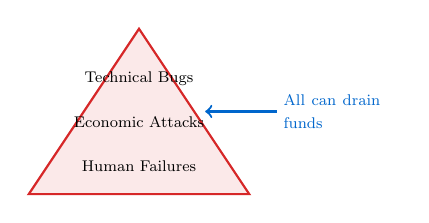
\begin{tikzpicture}[scale=0.7, transform shape]
% Risk pyramid
\draw[thick, dfred, fill=dfred!10] (0,0) -- (4,0) -- (2,3) -- cycle;
\node at (2,0.5) {\footnotesize Human Failures};
\node at (2,1.3) {\footnotesize Economic Attacks};
\node at (2,2.1) {\footnotesize Technical Bugs};
\draw[dfblue, thick, ->] (4.5,1.5) -- (3.2,1.5);
\node[right, text width=2cm] at (4.5,1.5) {\footnotesize \textcolor{dfblue}{All can drain funds}};
\end{tikzpicture}
\end{column}
\end{columns}

\vspace{3mm}
\begin{alertblock}{Key Mindset}
``Code is law'' until something goes wrong. Then we discover the limits of trustless systems.
\end{alertblock}
\end{frame}

% =============================================================================
% Frame 4 (NEW): Transition from Day 4
% =============================================================================
%% C5: Dedicated transition frame bridging Day 4 to Day 5
\begin{frame}{From Building to Breaking: Day 4 $\to$ Day 5}
\begin{center}
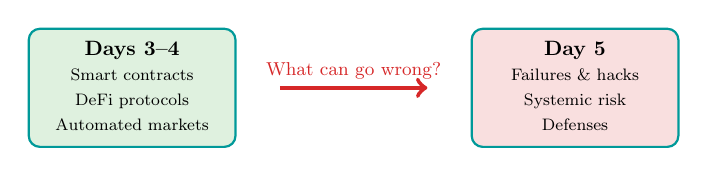
\begin{tikzpicture}[scale=0.75, transform shape]
% Day 4 box
\node[blockchain, minimum width=3.5cm, minimum height=2cm, fill=dfgreen!15] (day4) at (0,0) {
\begin{tabular}{c}
\textbf{Days 3--4}\\
\footnotesize Smart contracts\\
\footnotesize DeFi protocols\\
\footnotesize Automated markets
\end{tabular}
};

% Arrow
\draw[->, ultra thick, dfred] (2.5,0) -- (5,0) node[midway, above, font=\small] {What can go wrong?};

% Day 5 box
\node[blockchain, minimum width=3.5cm, minimum height=2cm, fill=dfred!15] (day5) at (7.5,0) {
\begin{tabular}{c}
\textbf{Day 5}\\
\footnotesize Failures \& hacks\\
\footnotesize Systemic risk\\
\footnotesize Defenses
\end{tabular}
};
\end{tikzpicture}
\end{center}

\vspace{5mm}
In Days 3--4 we learned how DeFi creates value through smart contracts and automated markets. Today we ask: \textbf{what happens when things go wrong?}

\vspace{3mm}
\begin{alertblock}{The Stakes Are Real}
Over \textbf{\$100 billion} has been lost to hacks, exploits, fraud, and collapses in digital finance. Understanding these failures is the key to understanding what makes---or breaks---the entire ecosystem.
\end{alertblock}
\end{frame}

% =============================================================================
% Frame 5: The Big Picture: Why Failures Matter
% =============================================================================
\begin{frame}{The Big Picture: Why Failures Matter}
\begin{center}
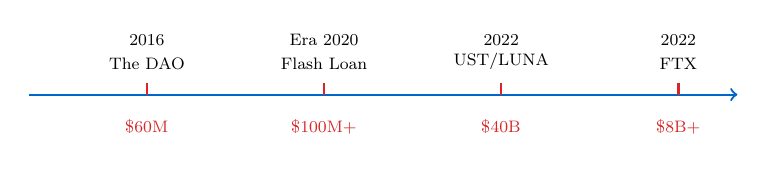
\begin{tikzpicture}[scale=0.75, transform shape]
% Timeline of major events
\draw[thick, dfblue, ->] (0,0) -- (12,0);

% Milestones
\node[above] at (2,0.3) {\footnotesize The DAO};
\node[above] at (2,0.7) {\footnotesize 2016};
\draw[thick, dfred] (2,0) -- (2,0.2);

\node[above] at (5,0.3) {\footnotesize Flash Loan};
\node[above] at (5,0.7) {\footnotesize Era 2020};
\draw[thick, dfred] (5,0) -- (5,0.2);

\node[above] at (8,0.3) {\footnotesize UST/LUNA};
\node[above] at (8,0.7) {\footnotesize 2022};
\draw[thick, dfred] (8,0) -- (8,0.2);

\node[above] at (11,0.3) {\footnotesize FTX};
\node[above] at (11,0.7) {\footnotesize 2022};
\draw[thick, dfred] (11,0) -- (11,0.2);

% Loss amounts
\node[below] at (2,-0.3) {\textcolor{dfred}{\footnotesize \$60M}};
\node[below] at (5,-0.3) {\textcolor{dfred}{\footnotesize \$100M+}};
\node[below] at (8,-0.3) {\textcolor{dfred}{\footnotesize \$40B}};
\node[below] at (11,-0.3) {\textcolor{dfred}{\footnotesize \$8B+}};
\end{tikzpicture}
\end{center}

\vspace{3mm}
\textbf{Cumulative losses in DeFi/crypto exceed \$100 billion.}

\vspace{2mm}
\begin{itemize}
\item Understanding failures is essential for building secure systems
\item Each exploit category teaches different lessons
\item Risk assessment requires knowing what can go wrong
\end{itemize}

\vspace{3mm}
\begin{block}{Course Context}
Day 5 examines the ``dark side''---failures, regulation, governance, and privacy. This topic focuses on what goes wrong technically and economically.
\end{block}
\end{frame}

% =============================================================================
% Frame 6: A Taxonomy of Failures
% =============================================================================
\begin{frame}{A Taxonomy of Failures}
\begin{center}
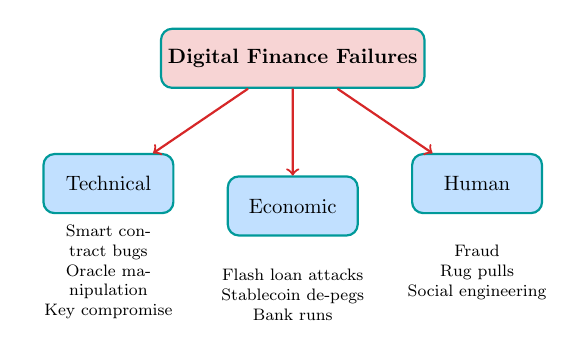
\begin{tikzpicture}[scale=0.75, transform shape]
% Main categories
\node (failures) [blockchain, minimum width=3cm, fill=dfred!20] {\textbf{Digital Finance Failures}};

\node (technical) [blockchain, below left of=failures, node distance=3cm, xshift=-1cm, minimum width=2.2cm] {Technical};
\node (economic) [blockchain, below of=failures, node distance=2.5cm, minimum width=2.2cm] {Economic};
\node (human) [blockchain, below right of=failures, node distance=3cm, xshift=1cm, minimum width=2.2cm] {Human};

% Arrows
\draw[->, thick, dfred] (failures) -- (technical);
\draw[->, thick, dfred] (failures) -- (economic);
\draw[->, thick, dfred] (failures) -- (human);

% Sub-categories
\node[below of=technical, node distance=1.5cm, font=\footnotesize, text width=2.5cm, align=center] {Smart contract bugs\\Oracle manipulation\\Key compromise};

\node[below of=economic, node distance=1.5cm, font=\footnotesize, text width=2.5cm, align=center] {Flash loan attacks\\Stablecoin de-pegs\\Bank runs};

\node[below of=human, node distance=1.5cm, font=\footnotesize, text width=2.5cm, align=center] {Fraud\\Rug pulls\\Social engineering};
\end{tikzpicture}
\end{center}

\vspace{3mm}
\textbf{Key Insight:} All three categories can result in total loss of funds, but they require different defenses.
\end{frame}

% =============================================================================
% Frame 7 (NEW): Navigation Roadmap
% =============================================================================
%% M9: Roadmap frame between taxonomy and deep dives
\begin{frame}{Roadmap: Where We Are Going}
\begin{center}
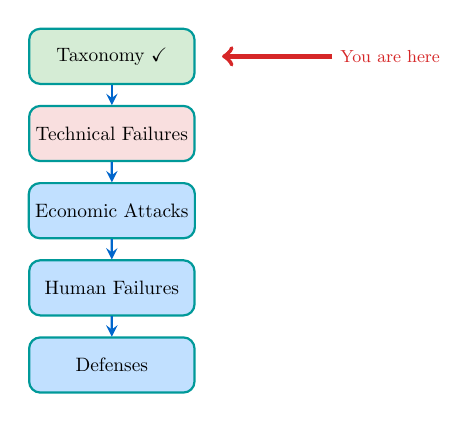
\begin{tikzpicture}[scale=0.7, transform shape, node distance=1.4cm]
% Steps
\node[blockchain, fill=dfgreen!20, minimum width=3cm] (tax) {Taxonomy \checkmark};
\node[blockchain, below of=tax, minimum width=3cm, fill=dfred!15] (tech) {Technical Failures};
\node[blockchain, below of=tech, minimum width=3cm] (econ) {Economic Attacks};
\node[blockchain, below of=econ, minimum width=3cm] (human) {Human Failures};
\node[blockchain, below of=human, minimum width=3cm] (defense) {Defenses};

\draw[arrow] (tax) -- (tech);
\draw[arrow] (tech) -- (econ);
\draw[arrow] (econ) -- (human);
\draw[arrow] (human) -- (defense);

% Current marker
\draw[->, ultra thick, dfred] (4,0) -- (2,0) node[pos=0, right, font=\small] {You are here};
\end{tikzpicture}
\end{center}

\vspace{3mm}
We will explore each category with \textbf{real-world case studies} and \textbf{everyday analogies} to make the concepts concrete. No coding knowledge is required.
\end{frame}

% =============================================================================
% Frame 8: Category 1: Technical Failures
% =============================================================================
%% H1--H6: Added plain-English definitions/analogies for all jargon items
\begin{frame}{Category 1: Technical Failures}
\begin{columns}[T]
\begin{column}{0.48\textwidth}
\textbf{Smart Contract Bugs:}
\begin{itemize}
\item Reentrancy attacks
\item Integer overflow/underflow (like a car odometer rolling from 999,999 back to 000,000)
\item Mistakes in the rules---like a vending machine that gives change before checking if you paid
\item Access control flaws (when the wrong people can use restricted features)
\end{itemize}

\vspace{3mm}
\textbf{Infrastructure Failures:}
\begin{itemize}
\item Oracle manipulation (the blockchain's ``window to the outside world''---we'll explain oracles in detail shortly)
\item Bridge vulnerabilities (bridges connect different blockchains---we'll explore their risks later)
\item Consensus bugs (errors in the agreement process between computers)
\item Key management failures
\end{itemize}
\end{column}
\begin{column}{0.48\textwidth}
\begin{alertblock}{The DAO Hack (2016)}
\textbf{Loss:} \$60M (3.6M ETH)\\
\textbf{Cause:} Reentrancy bug\\
\textbf{Result:} Ethereum hard fork\\
\textbf{Lesson:} Code is NOT always law
\end{alertblock}

\vspace{3mm}
\begin{block}{Wormhole Bridge (2022)}
\textbf{Loss:} \$320M\\
\textbf{Cause:} Signature verification bug\\
Attacker minted unbacked tokens
\end{block}
\end{column}
\end{columns}
\end{frame}

% =============================================================================
% Frame 9: Deep Dive: Reentrancy Attack
% =============================================================================
%% H12: Added bank teller analogy for reentrancy
\begin{frame}{Deep Dive: Reentrancy Attack}
\begin{center}
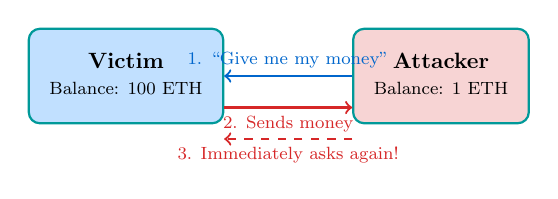
\begin{tikzpicture}[scale=0.8, transform shape, node distance=2cm]
% Victim contract
\node (victim) [blockchain, minimum width=2.5cm, minimum height=1.5cm] {
\begin{tabular}{c}
\textbf{Victim}\\
\footnotesize Balance: 100 ETH
\end{tabular}
};

% Attacker contract
\node (attacker) [blockchain, right of=victim, node distance=5cm, minimum width=2.5cm, minimum height=1.5cm, fill=dfred!20] {
\begin{tabular}{c}
\textbf{Attacker}\\
\footnotesize Balance: 1 ETH
\end{tabular}
};

% Steps
\draw[->, thick, dfblue] (attacker.west) -- node[above, font=\footnotesize] {1. ``Give me my money''} (victim.east);
\draw[->, thick, dfred] ([yshift=-5mm]victim.east) -- node[below, font=\footnotesize] {2. Sends money} ([yshift=-5mm]attacker.west);
\draw[->, thick, dfred, dashed] ([yshift=-10mm]attacker.west) -- node[below, font=\footnotesize] {3. Immediately asks again!} ([yshift=-10mm]victim.east);

\end{tikzpicture}
\end{center}

\vspace{3mm}
\textbf{Analogy:} Imagine a bank teller who hands you cash and THEN checks your balance. A clever attacker keeps asking for cash before the teller finishes checking---getting paid multiple times from one withdrawal.

\vspace{2mm}
\textbf{The Problem:}
\begin{enumerate}
\item Victim sends money \textit{before} updating the balance record
\item Attacker immediately requests another withdrawal
\item Balance not yet updated, so the check passes again
\item Repeat until the entire contract is drained
\end{enumerate}

\begin{block}{Prevention}
Check-Effects-Interactions pattern: Update records BEFORE sending money.
\end{block}
\end{frame}

% =============================================================================
% Frame 10: Vulnerable vs. Safe --- Plain English
% =============================================================================
%% C2, C3: Replaced Solidity code with plain-English pseudocode
%% H16: Added note that no code reading is required
\begin{frame}{Vulnerable vs. Safe: How the Fix Works}

\begin{alertblock}{No Code Required}
You don't need to understand programming---focus on the \textbf{order of steps} below.
\end{alertblock}

\begin{columns}[T]
\begin{column}{0.48\textwidth}
\textbf{\textcolor{dfred}{Dangerous Order:}}
\begin{enumerate}
\item Check: ``Does this person have money?''
\item \textcolor{dfred}{\textbf{Send the money out}} $\leftarrow$ external call
\item Update records: ``They now have \$0''
\end{enumerate}

\vspace{3mm}
\textbf{Why it fails:} The contract sends money BEFORE updating its records---this is the vulnerability. The attacker can keep requesting money before step 3 ever runs.
\end{column}
\begin{column}{0.48\textwidth}
\textbf{\textcolor{dfgreen}{Safe Order:}}
\begin{enumerate}
\item Check: ``Does this person have money?''
\item \textcolor{dfgreen}{\textbf{Update records first}}: ``They now have \$0''
\item Send the money out
\end{enumerate}

\vspace{3mm}
\textbf{Why it works:} Even if the attacker tries to re-enter, the records already show \$0, so the check in step 1 fails.
\end{column}
\end{columns}

\vspace{3mm}
\begin{block}{Check-Effects-Interactions (CEI) Pattern}
\begin{enumerate}
\item \textbf{Check:} Validate conditions (``Do they have enough?'')
\item \textbf{Effects:} Update your own records
\item \textbf{Interactions:} Only THEN send money or talk to other contracts
\end{enumerate}
\end{block}
\end{frame}

% =============================================================================
% Frame 11: Integer Overflow and Underflow
% =============================================================================
%% C6, H7: Replaced 2^{256}-1 with simple uint8 (0--255) example
\begin{frame}{Integer Overflow and Underflow}
\begin{columns}[T]
\begin{column}{0.52\textwidth}
\textbf{The Problem:}

\textbf{Analogy:} Imagine a counter that can only store numbers 0 to 255. What happens when you add 1 to 255? It wraps around to 0---that's \textbf{overflow}. What happens when you subtract 1 from 0? It wraps to 255---that's \textbf{underflow}.

\vspace{3mm}
Older smart contracts used counters like this but with much bigger numbers. Attackers exploited the wrapping to give themselves enormous fake balances.

\vspace{3mm}
\textbf{Example:}
\begin{itemize}
\item Attacker's balance = 0 tokens
\item Attacker subtracts 1 token
\item Balance wraps to a gigantic number
\item Attacker now has ``infinite'' tokens!
\end{itemize}
\end{column}
\begin{column}{0.45\textwidth}
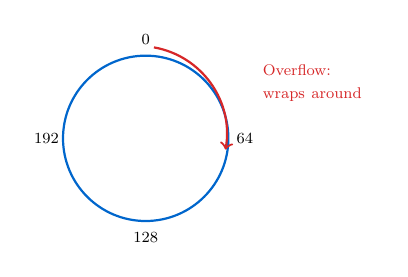
\begin{tikzpicture}[scale=0.7, transform shape]
% Number line wrapping
\draw[thick, dfblue] (0,0) circle (1.5cm);
\node at (0,1.8) {\footnotesize 0};
\node at (1.8,0) {\footnotesize 64};
\node at (0,-1.8) {\footnotesize 128};
\node at (-1.8,0) {\footnotesize 192};

% Arrows showing wrap
\draw[->, thick, dfred] (0.15,1.65) arc (80:-10:1.6);
\node[right, text width=2cm] at (2,1) {\footnotesize \textcolor{dfred}{Overflow: wraps around}};
\end{tikzpicture}

\vspace{3mm}
\begin{block}{Solution}
Modern smart contracts include automatic checks that stop the transaction if a number would wrap around.
\end{block}
\end{column}
\end{columns}
\end{frame}

% =============================================================================
% Frame 12: Access Control Vulnerabilities
% =============================================================================
%% C2: Replaced Solidity code with plain-English descriptions
\begin{frame}{Access Control Vulnerabilities}
\begin{columns}[T]
\begin{column}{0.48\textwidth}
\textbf{Common Mistakes:}
\begin{itemize}
\item No check on \textit{who} is calling a function
\item Features meant to be private are left open to anyone
\item Administrative powers not properly restricted
\item Setup steps left unprotected
\end{itemize}

\vspace{3mm}
\textbf{\textcolor{dfred}{Vulnerable} (no lock on the door):}
\begin{itemize}
\item Anyone can call ``change the owner''
\item Attacker makes \textit{themselves} the owner
\item Attacker now controls the entire contract
\end{itemize}
\end{column}
\begin{column}{0.48\textwidth}
\textbf{\textcolor{dfgreen}{Safe} (locked door):}
\begin{itemize}
\item Before running ``change the owner,'' the contract checks: ``Is the person asking \textit{actually} the current owner?''
\item If not, the request is rejected
\item Only the real owner can transfer control
\end{itemize}

\vspace{3mm}
\textbf{Analogy:} Think of a house where the front door has no lock. Anyone can walk in and claim they own it. Adding access control is like installing a lock---only people with the right key can get in.

\vspace{3mm}
\begin{alertblock}{Best Practice}
Every sensitive function should check ``who is asking?'' before executing.
\end{alertblock}
\end{column}
\end{columns}
\end{frame}

% =============================================================================
% Frame 13 (NEW): Pause & Reflect
% =============================================================================
%% C4: Breathing room after dense technical frames
\begin{frame}{Pause \& Reflect}
\begin{center}
\textbf{\Large Let's take stock of what we've covered so far.}
\end{center}

\vspace{5mm}
We've seen three types of \textbf{technical} vulnerabilities:

\begin{enumerate}
\item \textbf{Reentrancy} --- the ``ask-for-money-before-records-update'' trick
\item \textbf{Integer overflow/underflow} --- the ``odometer wrapping around'' problem
\item \textbf{Access control flaws} --- the ``unlocked front door'' problem
\end{enumerate}

\vspace{5mm}
\begin{block}{Discussion Question}
Which of these three do you think is the most dangerous, and why? Consider: which one is hardest to detect, and which one has caused the biggest losses?
\end{block}

\vspace{5mm}
\textbf{Coming up next:} Economic attacks---where the code works exactly as written, but attackers find clever ways to exploit the \textit{design} itself.
\end{frame}

% =============================================================================
% Frame 14: Category 2: Economic Attacks
% =============================================================================
%% H13: Added flash loan atomicity analogy
%% M2: Added atomicity definition before use
\begin{frame}{Category 2: Economic Attacks}
\begin{columns}[T]
\begin{column}{0.48\textwidth}
\textbf{Flash Loan Attacks:}

\textbf{Analogy:} Think of a flash loan like a time-travel movie: you can borrow millions, use them, and return them---all in a single instant. If anything goes wrong, it's as if it never happened.

\begin{itemize}
\item Borrow millions, attack, repay---all in one transaction
\item No collateral needed
\item Exploit price discrepancies
\item Manipulate governance votes
\end{itemize}

\vspace{3mm}
\textbf{How Flash Loans Work:}

``Atomic'' means all-or-nothing: either \textit{every} step succeeds, or the entire transaction is cancelled as if it never happened.

\begin{enumerate}
\item Borrow \$100M (no collateral)
\item Execute attack strategy
\item Repay \$100M + small fee
\item If any step fails, everything is reversed
\end{enumerate}
\end{column}
\begin{column}{0.48\textwidth}
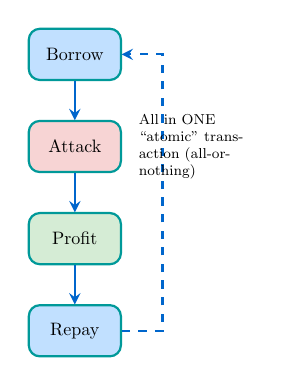
\begin{tikzpicture}[scale=0.65, transform shape, node distance=1.8cm]
% Flash loan cycle
\node (borrow) [blockchain, minimum width=1.8cm] {Borrow};
\node (attack) [blockchain, below of=borrow, minimum width=1.8cm, fill=dfred!20] {Attack};
\node (profit) [blockchain, below of=attack, minimum width=1.8cm, fill=dfgreen!20] {Profit};
\node (repay) [blockchain, below of=profit, minimum width=1.8cm] {Repay};

\draw[arrow] (borrow) -- (attack);
\draw[arrow] (attack) -- (profit);
\draw[arrow] (profit) -- (repay);
\draw[arrow, dashed] (repay.east) -- ++(0.8,0) |- (borrow.east);

\node[right of=attack, node distance=2.5cm, font=\footnotesize, text width=2.5cm] {All in ONE ``atomic'' transaction (all-or-nothing)};
\end{tikzpicture}
\end{column}
\end{columns}
\end{frame}

% =============================================================================
% Frame 15: Flash Loan Attack Example: bZx (2020)
% =============================================================================
%% C6, H8: Added definition of "shorting" before it appears
\begin{frame}{Flash Loan Attack Example: bZx (2020)}

\begin{block}{Key Term: Shorting}
\textbf{Shorting} means betting that a price will go \textbf{down}. If Alice thinks Bitcoin will drop from \$50,000 to \$40,000, she can ``short'' it and profit if she's right. If the price goes up instead, she loses money.
\end{block}

\begin{center}
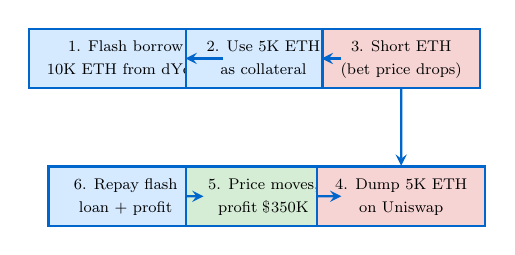
\begin{tikzpicture}[scale=0.7, transform shape, node distance=2.5cm]
% Steps
\node (step1) [process, minimum width=2.8cm, minimum height=1cm] {
\begin{tabular}{c}
\footnotesize 1. Flash borrow\\
\footnotesize 10K ETH from dYdX
\end{tabular}
};

\node (step2) [process, right of=step1, minimum width=2.8cm, minimum height=1cm] {
\begin{tabular}{c}
\footnotesize 2. Use 5K ETH\\
\footnotesize as collateral
\end{tabular}
};

\node (step3) [process, right of=step2, minimum width=2.8cm, minimum height=1cm, fill=dfred!20] {
\begin{tabular}{c}
\footnotesize 3. Short ETH\\
\footnotesize (bet price drops)
\end{tabular}
};

\node (step4) [process, below of=step1, minimum width=2.8cm, minimum height=1cm] {
\begin{tabular}{c}
\footnotesize 6. Repay flash\\
\footnotesize loan + profit
\end{tabular}
};

\node (step5) [process, below of=step2, minimum width=2.8cm, minimum height=1cm, fill=dfgreen!20] {
\begin{tabular}{c}
\footnotesize 5. Price moves,\\
\footnotesize profit \$350K
\end{tabular}
};

\node (step6) [process, below of=step3, minimum width=2.8cm, minimum height=1cm, fill=dfred!20] {
\begin{tabular}{c}
\footnotesize 4. Dump 5K ETH\\
\footnotesize on Uniswap
\end{tabular}
};

% Arrows
\draw[arrow] (step1) -- (step2);
\draw[arrow] (step2) -- (step3);
\draw[arrow] (step3) -- (step6);
\draw[arrow] (step6) -- (step5);
\draw[arrow] (step5) -- (step4);
\end{tikzpicture}
\end{center}

\vspace{3mm}
\textbf{Key insight:} Capital requirement to manipulate markets dropped from millions to \textbf{zero}.
\end{frame}

% =============================================================================
% Frame 16: The Atomic Property of Flash Loans
% =============================================================================
\begin{frame}{The Atomic Property of Flash Loans}
\begin{columns}[T]
\begin{column}{0.55\textwidth}
\textbf{What ``atomic'' means:}
\begin{itemize}
\item All operations must complete in ONE transaction
\item Either everything succeeds, or nothing happens
\item Loan + use + repay = single block
\item No collateral at risk (transaction reverses if unpaid)
\end{itemize}

\vspace{3mm}
\textbf{Why this enables attacks:}
\begin{itemize}
\item Zero capital requirement
\item No personal funds at risk
\item Can borrow unlimited amounts
\item Only pay small fee if attack succeeds
\end{itemize}
\end{column}
\begin{column}{0.42\textwidth}
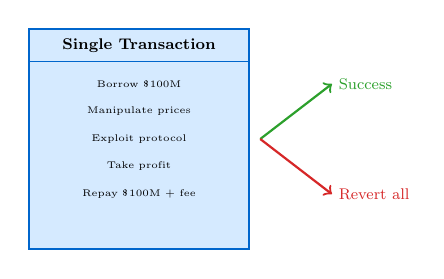
\begin{tikzpicture}[scale=0.7, transform shape]
% Transaction box
\draw[thick, dfblue, fill=dflightblue4] (0,0) rectangle (4,4);
\node at (2,3.7) {\footnotesize \textbf{Single Transaction}};
\draw[dfblue] (0,3.4) -- (4,3.4);

% Steps inside
\node at (2,3) {\tiny Borrow \$100M};
\node at (2,2.5) {\tiny Manipulate prices};
\node at (2,2) {\tiny Exploit protocol};
\node at (2,1.5) {\tiny Take profit};
\node at (2,1) {\tiny Repay \$100M + fee};

% Success/fail
\draw[->, thick, dfgreen] (4.2,2) -- (5.5,3);
\node[right] at (5.5,3) {\footnotesize \textcolor{dfgreen}{Success}};

\draw[->, thick, dfred] (4.2,2) -- (5.5,1);
\node[right] at (5.5,1) {\footnotesize \textcolor{dfred}{Revert all}};
\end{tikzpicture}
\end{column}
\end{columns}

\begin{alertblock}{Democratization of Capital}
Flash loans ``democratize'' access to large capital---for both legitimate arbitrage AND attacks.
\end{alertblock}
\end{frame}

% =============================================================================
% Frame 17: Oracle Manipulation
% =============================================================================
%% M6: Added "thermometer that lies" analogy for oracle manipulation
%% M3: Added parenthetical recall for DEX/spot price
\begin{frame}{Oracle Manipulation}
\begin{columns}[T]
\begin{column}{0.55\textwidth}
\textbf{The Problem:}

\textbf{Analogy:} An oracle is like a thermometer for the blockchain---it reports real-world information (like prices) that smart contracts cannot see on their own. \textbf{Oracle manipulation} is like tampering with that thermometer so it shows a wrong temperature, causing the system to make bad decisions.

\begin{itemize}
\item DeFi protocols need external price data
\item Oracles provide this data on-chain
\item If oracle can be manipulated, protocol is vulnerable
\end{itemize}

\vspace{3mm}
\textbf{Attack Pattern:}
\begin{enumerate}
\item Flash borrow large amount
\item Trade on a DEX (decentralized exchange---recall from Day 4) to move the current ``spot'' price
\item Protocol reads the manipulated price
\item Exploit (borrow more, liquidate others)
\item Restore price, repay loan
\end{enumerate}
\end{column}
\begin{column}{0.42\textwidth}
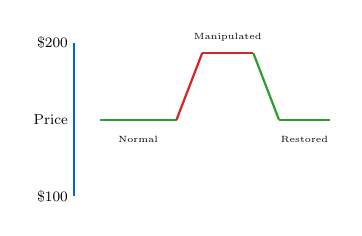
\begin{tikzpicture}[scale=0.65, transform shape]
% Normal price
\draw[thick, dfblue] (0,0) -- (0,3);
\node[left] at (0,0) {\footnotesize \$100};
\node[left] at (0,1.5) {\footnotesize Price};
\node[left] at (0,3) {\footnotesize \$200};

% Price line
\draw[thick, dfgreen] (0.5,1.5) -- (2,1.5);
\draw[thick, dfred] (2,1.5) -- (2.5,2.8);
\draw[thick, dfred] (2.5,2.8) -- (3.5,2.8);
\draw[thick, dfgreen] (3.5,2.8) -- (4,1.5);
\draw[thick, dfgreen] (4,1.5) -- (5,1.5);

% Labels
\node[below] at (1.25,1.3) {\tiny Normal};
\node[above] at (3,2.9) {\tiny Manipulated};
\node[below] at (4.5,1.3) {\tiny Restored};
\end{tikzpicture}

\vspace{5mm}
\begin{block}{Defense}
Use TWAP (Time-Weighted Average Price) or decentralized oracles like Chainlink.
\end{block}
\end{column}
\end{columns}
\end{frame}

% =============================================================================
% Frame 18: Spot Price vs. TWAP Oracles
% =============================================================================
\begin{frame}{Spot Price vs. TWAP Oracles}
\begin{columns}[T]
\begin{column}{0.48\textwidth}
\textbf{Spot Price Oracle:}
\begin{itemize}
\item Current instant price
\item Single data source (one DEX)
\item Easy to manipulate with one trade
\item Cheap and simple
\end{itemize}

\vspace{3mm}
\textbf{Vulnerability:}
\begin{itemize}
\item Flash loan can move price
\item Manipulation in single block
\item No historical context
\end{itemize}
\end{column}
\begin{column}{0.48\textwidth}
\textbf{TWAP Oracle:}
\begin{itemize}
\item Time-Weighted Average Price
\item Average over time window (e.g., 30 min)
\item Resistant to short-term manipulation
\item More expensive to attack
\end{itemize}

\vspace{3mm}
\textbf{Why it's safer:}
\begin{itemize}
\item Attacker must sustain manipulation
\item Across many blocks
\item Capital locked (not flash loan)
\end{itemize}
\end{column}
\end{columns}

\vspace{3mm}
\begin{alertblock}{Best Practice}
Use decentralized oracles (Chainlink) with multiple data sources and TWAP for price-sensitive operations.
\end{alertblock}
\end{frame}

% =============================================================================
% Frame 19: Category 3: Stablecoin Failures
% =============================================================================
%% H9: Added 2--3 sentence refresher on algorithmic stablecoins from Day 4
%% L4: Added "bank run" analogy for death spiral
\begin{frame}{Category 3: Stablecoin Failures}
\begin{columns}[T]
\begin{column}{0.55\textwidth}
\textbf{UST/LUNA Collapse (May 2022):}

\textit{Recall from Day 4:} Algorithmic stablecoins try to maintain their \$1 price through automatic mint/burn mechanisms rather than holding dollar reserves. UST was the largest such experiment.

\begin{itemize}
\item Market cap: \$18B at peak
\item De-pegged from \$1 to \$0.10
\item LUNA: \$80 to \$0.0001
\item Total value destroyed: \$40B+
\end{itemize}

\vspace{3mm}
\textbf{The Death Spiral:}

\textbf{Analogy:} This is similar to a traditional \textbf{bank run}---when everyone tries to withdraw at once, the system cannot handle it and collapses.

\begin{enumerate}
\item Large UST sell-off
\item Peg breaks, panic ensues
\item LUNA minted to defend peg
\item LUNA hyperinflates
\item Both collapse to zero
\end{enumerate}
\end{column}
\begin{column}{0.42\textwidth}
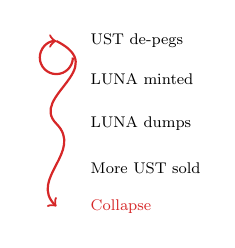
\begin{tikzpicture}[scale=0.7, transform shape]
% Death spiral
\draw[thick, dfred, ->] (0,3) .. controls (1,2.5) and (-0.5,2) .. (0,1.5) .. controls (0.5,1) and (-0.5,0.5) .. (0,0);

\node[right] at (0.5,3) {\footnotesize UST de-pegs};
\node[right] at (0.5,2.3) {\footnotesize LUNA minted};
\node[right] at (0.5,1.5) {\footnotesize LUNA dumps};
\node[right] at (0.5,0.7) {\footnotesize More UST sold};
\node[right] at (0.5,0) {\footnotesize \textcolor{dfred}{Collapse}};

% Spiral arrow indicating loop
\draw[thick, dfred, ->] (0.3,2.7) arc (0:-270:0.3);
\end{tikzpicture}

\vspace{3mm}
\begin{alertblock}{Lesson}
Algorithmic stability requires robust mechanisms---``code'' alone is insufficient.
\end{alertblock}
\end{column}
\end{columns}
\end{frame}

% =============================================================================
% Frame 20: Category 4: Centralized Exchange Collapses
% =============================================================================
%% M8: Added definition of "proof of reserves"
%% L3: Added relatable comparison for dollar amounts
\begin{frame}{Category 4: Centralized Exchange Collapses}
\begin{columns}[T]
\begin{column}{0.48\textwidth}
\textbf{FTX Collapse (Nov 2022):}
\begin{itemize}
\item 2nd largest crypto exchange
\item \$32B valuation (more than many national airlines)
\item Customer funds misappropriated
\item \$8B+ missing
\item CEO convicted of fraud
\end{itemize}

\vspace{3mm}
\textbf{Mt. Gox (2014):}
\begin{itemize}
\item 70\% of Bitcoin trading
\item 850,000 BTC ``lost''
\item Combination of hack + fraud
\item 10+ years to partial recovery
\end{itemize}
\end{column}
\begin{column}{0.48\textwidth}
\textbf{Common Patterns:}
\begin{enumerate}
\item Opaque operations
\item Commingled funds
\item Lack of proof of reserves (a public demonstration that the exchange actually holds all the assets it claims to hold)
\item Regulatory arbitrage
\item Charismatic founders
\end{enumerate}

\vspace{3mm}
\begin{alertblock}{Not Your Keys, Not Your Coins}
Centralized custodians reintroduce the trust problems DeFi was designed to solve.
\end{alertblock}
\end{column}
\end{columns}
\end{frame}

% =============================================================================
% Frame 21: Category 5: Rug Pulls and Fraud
% =============================================================================
%% M4: Added parenthetical recall for LP tokens
\begin{frame}{Category 5: Rug Pulls and Fraud}
\begin{columns}[T]
\begin{column}{0.55\textwidth}
\textbf{Types of Rug Pulls:}
\begin{itemize}
\item \textbf{Liquidity pull:} Developers drain LP tokens (recall: LP tokens represent your share of a liquidity pool)
\item \textbf{Limiting sell orders:} Hidden code prevents selling
\item \textbf{Dumping:} Team sells massive holdings
\item \textbf{Exit scam:} Project disappears with funds
\end{itemize}

\vspace{3mm}
\textbf{Red Flags:}
\begin{itemize}
\item Anonymous team
\item Unlocked liquidity
\item No audit
\item Unrealistic promises
\item FOMO marketing
\item Celebrity endorsements
\end{itemize}
\end{column}
\begin{column}{0.42\textwidth}
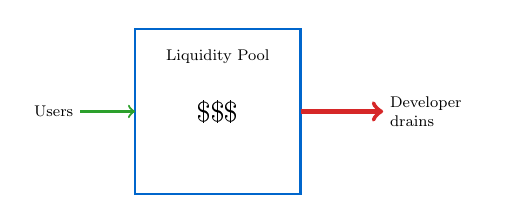
\begin{tikzpicture}[scale=0.7, transform shape]
% Rug pull diagram
\draw[thick, dfblue] (0,0) -- (0,3) -- (3,3) -- (3,0) -- cycle;
\node at (1.5,2.5) {\footnotesize Liquidity Pool};

% Users depositing
\draw[->, thick, dfgreen] (-1,1.5) -- (0,1.5);
\node[left, font=\footnotesize] at (-1,1.5) {Users};

% Rug pull
\draw[->, ultra thick, dfred] (3,1.5) -- (4.5,1.5);
\node[right, font=\footnotesize, text width=1.5cm] at (4.5,1.5) {Developer drains};

% Money icons
\node at (1.5,1.5) {\Large \$\$\$};
\end{tikzpicture}

\vspace{5mm}
\textbf{2021 Stats:}\\
\$2.8B lost to rug pulls (that's roughly the entire GDP of a small country)\\
(Chainalysis)
\end{column}
\end{columns}
\end{frame}

% =============================================================================
% Frame 22: Bridge Exploits - The Biggest Target
% =============================================================================
%% M7: Added "ferry between islands" analogy for bridge exploits
%% M5: Expanded TVL definition
\begin{frame}{Bridge Exploits --- The Biggest Target}
\begin{columns}[T]
\begin{column}{0.55\textwidth}
\textbf{Analogy:} A blockchain bridge is like a \textbf{ferry between islands}. Each island (blockchain) has its own currency. The ferry (bridge) locks your currency on one island and gives you equivalent currency on the other. If pirates (hackers) take over the ferry, they can steal everything on board.

\vspace{3mm}
\textbf{Why bridges are vulnerable:}
\begin{itemize}
\item Hold massive TVL (Total Value Locked---the total amount of assets deposited into the bridge)
\item Complex multi-chain logic
\item Multiple attack surfaces
\item Validator key management
\item Novel, less-tested code
\end{itemize}
\end{column}
\begin{column}{0.42\textwidth}
\textbf{Major Bridge Hacks:}

\vspace{2mm}
\begin{tabular}{lr}
\hline
\textbf{Bridge} & \textbf{Loss} \\
\hline
Ronin & \$625M \\
Poly Network & \$611M \\
Wormhole & \$320M \\
Nomad & \$190M \\
Harmony & \$100M \\
\hline
\end{tabular}

\vspace{5mm}
\begin{alertblock}{2022 Pattern}
Bridges accounted for 69\% of crypto stolen in 2022.
\end{alertblock}
\end{column}
\end{columns}
\end{frame}

% =============================================================================
% Frame 23: Systemic Risk in Digital Finance
% =============================================================================
%% L1: Added re-definition of composability
\begin{frame}{Systemic Risk in Digital Finance}
\begin{center}
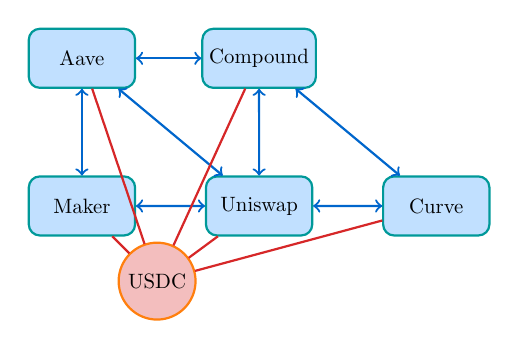
\begin{tikzpicture}[scale=0.75, transform shape]
% Interconnected protocols
\node (aave) [blockchain, minimum width=1.8cm] {Aave};
\node (compound) [blockchain, right of=aave, node distance=3cm, minimum width=1.8cm] {Compound};
\node (maker) [blockchain, below of=aave, node distance=2.5cm, minimum width=1.8cm] {Maker};
\node (uniswap) [blockchain, below of=compound, node distance=2.5cm, minimum width=1.8cm] {Uniswap};
\node (curve) [blockchain, right of=uniswap, node distance=3cm, minimum width=1.8cm] {Curve};

% Connections
\draw[thick, dfblue, <->] (aave) -- (compound);
\draw[thick, dfblue, <->] (aave) -- (maker);
\draw[thick, dfblue, <->] (compound) -- (uniswap);
\draw[thick, dfblue, <->] (maker) -- (uniswap);
\draw[thick, dfblue, <->] (uniswap) -- (curve);
\draw[thick, dfblue, <->] (aave) -- (uniswap);
\draw[thick, dfblue, <->] (compound) -- (curve);

% Stablecoins at center
\node (usdc) [transaction, below right of=maker, node distance=1.8cm, fill=dfred!30] {USDC};
\draw[thick, dfred] (usdc) -- (aave);
\draw[thick, dfred] (usdc) -- (compound);
\draw[thick, dfred] (usdc) -- (maker);
\draw[thick, dfred] (usdc) -- (uniswap);
\draw[thick, dfred] (usdc) -- (curve);
\end{tikzpicture}
\end{center}

\vspace{3mm}
\textbf{DeFi Composability (recall: building blocks that connect together) = Systemic Risk:}
\begin{itemize}
\item Protocols depend on each other (``money legos'')
\item Stablecoins are systemic (USDC freeze = cascade)
\item Oracle failure affects ALL dependent protocols
\item Smart contract bug can propagate through ecosystem
\end{itemize}
\end{frame}

% =============================================================================
% Frame 24: Largest DeFi Exploits (2020-2024)
% =============================================================================
\begin{frame}{Largest DeFi Exploits (2020--2024)}
\begin{center}
\renewcommand{\arraystretch}{1.3}
\begin{tabular}{|l|r|l|l|}
\hline
\textbf{Protocol} & \textbf{Loss} & \textbf{Type} & \textbf{Year} \\
\hline
Ronin Bridge & \$625M & Bridge exploit & 2022 \\
\hline
Poly Network & \$611M & Bridge exploit & 2021 \\
\hline
FTX & \$477M & Hack post-bankruptcy & 2022 \\
\hline
Wormhole & \$320M & Bridge exploit & 2022 \\
\hline
Nomad Bridge & \$190M & Bridge exploit & 2022 \\
\hline
Beanstalk & \$182M & Flash loan governance & 2022 \\
\hline
Wintermute & \$160M & Key compromise & 2022 \\
\hline
\end{tabular}
\end{center}

\vspace{3mm}
\begin{alertblock}{Pattern Recognition}
\textbf{Bridges are the weakest link.} Cross-chain bridges hold massive amounts of locked assets but have complex attack surfaces.
\end{alertblock}
\end{frame}

% =============================================================================
% Frame 25: Defense Patterns: ReentrancyGuard
% =============================================================================
%% H10: Replaced Solidity code with "door lock" diagram
%% L2: Replaced "mutex" with "lock"
\begin{frame}{Defense Patterns: Reentrancy Guard}
\begin{columns}[T]
\begin{column}{0.52\textwidth}
\textbf{The Door Lock Pattern:}

\textbf{Analogy:} When you enter a bathroom, you lock the door. If someone else tries to enter while you're inside, the lock stops them. Once you're done, you unlock it. A reentrancy guard works exactly the same way.

\vspace{3mm}
\begin{center}
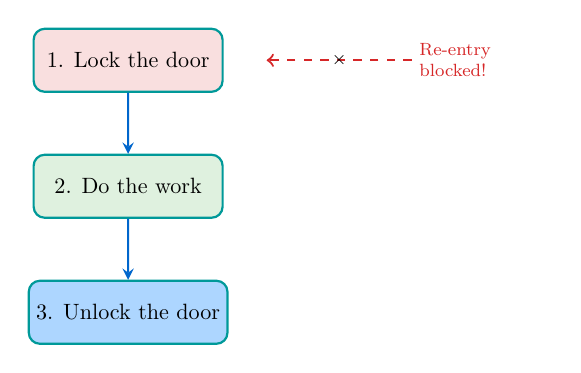
\begin{tikzpicture}[scale=0.8, transform shape, node distance=2cm]
% Three steps
\node[blockchain, fill=dfred!15, minimum width=3cm] (lock) {1. Lock the door};
\node[blockchain, below of=lock, minimum width=3cm, fill=dfgreen!15] (work) {2. Do the work};
\node[blockchain, below of=work, minimum width=3cm, fill=dflightblue2] (unlock) {3. Unlock the door};

\draw[arrow] (lock) -- (work);
\draw[arrow] (work) -- (unlock);

% Blocked re-entry
\draw[->, thick, dfred, dashed] (4.5,0) -- (2.2,0);
\node[right, font=\footnotesize, text width=2cm] at (4.5,0) {\textcolor{dfred}{Re-entry blocked!}};
\node at (3.35,0) {\footnotesize $\times$};
\end{tikzpicture}
\end{center}
\end{column}
\begin{column}{0.45\textwidth}
\textbf{How it works:}
\begin{enumerate}
\item Set the lock when someone enters
\item If a re-entrant call tries to enter...
\item The lock is still set, so the call is rejected
\item Lock released only when the original operation finishes
\end{enumerate}

\vspace{3mm}
\begin{block}{Best Practice}
Production smart contracts use well-tested, pre-built reentrancy guard libraries (e.g., from OpenZeppelin) rather than writing their own.
\end{block}
\end{column}
\end{columns}
\end{frame}

% =============================================================================
% Frame 26: Defense Patterns: Pull vs. Push
% =============================================================================
%% H11: Replaced Solidity code with waiter/buffet analogy
\begin{frame}{Defense Patterns: Pull vs. Push Payments}
\begin{columns}[T]
\begin{column}{0.48\textwidth}
\textbf{Push Pattern (Risky):}

\textbf{Analogy:} A waiter brings food to every table. If one table is blocked (a difficult customer), the waiter is stuck and nobody else gets served.

\vspace{3mm}
\textbf{How it works:}
\begin{itemize}
\item The contract sends money to each user one by one
\item If one recipient fails (bad address, malicious contract), the \textit{entire} payment process stops
\end{itemize}

\vspace{3mm}
\textbf{Problems:}
\begin{itemize}
\item One bad recipient blocks all others
\item Reentrancy risk
\item Can run out of processing power (``gas'')
\end{itemize}
\end{column}
\begin{column}{0.48\textwidth}
\textbf{Pull Pattern (Safe):}

\textbf{Analogy:} A buffet---everyone goes up and serves themselves when they're ready. If one person has trouble, it doesn't affect anyone else.

\vspace{3mm}
\textbf{How it works:}
\begin{itemize}
\item The contract records how much each user is owed
\item Users come and withdraw their own funds whenever they want
\item Each withdrawal is independent
\end{itemize}

\vspace{3mm}
\textbf{Benefits:}
\begin{itemize}
\item Isolates failures
\item User controls timing
\item Easier to secure
\end{itemize}
\end{column}
\end{columns}

\vspace{3mm}
\begin{alertblock}{Rule of Thumb}
Let users ``pull'' funds rather than ``pushing'' to them---like a buffet instead of table service.
\end{alertblock}
\end{frame}

% =============================================================================
% Frame 27: Defense in Depth
% =============================================================================
\begin{frame}{Defense in Depth}
\begin{center}
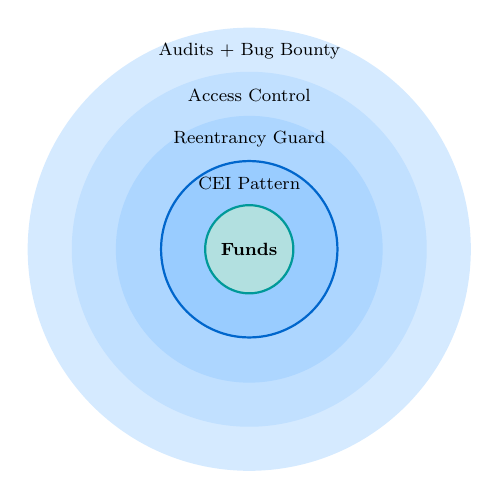
\begin{tikzpicture}[scale=0.8, transform shape]
% Concentric circles representing layers
\draw[thick, dflightblue4, fill=dflightblue4] (0,0) circle (3.5cm);
\draw[thick, dflightblue3, fill=dflightblue3] (0,0) circle (2.8cm);
\draw[thick, dflightblue2, fill=dflightblue2] (0,0) circle (2.1cm);
\draw[thick, dfblue, fill=dflightblue] (0,0) circle (1.4cm);
\draw[thick, dfteal, fill=dfteal!30] (0,0) circle (0.7cm);

% Labels
\node at (0,0) {\footnotesize \textbf{Funds}};
\node at (0,1.05) {\footnotesize CEI Pattern};
\node at (0,1.75) {\footnotesize Reentrancy Guard};
\node at (0,2.45) {\footnotesize Access Control};
\node at (0,3.15) {\footnotesize Audits + Bug Bounty};
\end{tikzpicture}
\end{center}

\vspace{3mm}
\textbf{Defense in Depth Principle:}
\begin{itemize}
\item Multiple independent security layers
\item If one layer fails, others still protect
\item No single point of failure
\end{itemize}
\end{frame}

% =============================================================================
% Frame 28: Hands-On Exercise I
% =============================================================================
\begin{frame}{Hands-On: Analyzing an Exploit (NB11)}
\begin{center}
\textbf{\Large Simulate Real Exploit Scenarios}
\end{center}

\vspace{5mm}
\textbf{In the Colab notebook, we will:}
\begin{enumerate}
\item Run simulations of exploit scenarios (reentrancy, flash loans, oracle manipulation)
\item Model how each attack type drains funds step-by-step
\item Identify the attack patterns and vulnerabilities
\item Calculate attacker profit in simulated scenarios
\item Discuss what could have prevented each exploit
\end{enumerate}

\vspace{5mm}
\begin{block}{Access the Notebook}
\texttt{day\_05/notebooks/NB11\_DeFi\_Exploits.ipynb}

\vspace{2mm}
\footnotesize We'll simulate real exploit types to understand how they work. All code is pre-written---you interact with it, not write it.
\end{block}

\bottomnote{Time: 20-25 minutes for guided exploration}
\end{frame}

% =============================================================================
% Frame 29: Hands-On Exercise II - What You'll Learn
% =============================================================================
\begin{frame}{Notebook Objectives}
\begin{columns}[T]
\begin{column}{0.48\textwidth}
\textbf{Part 1: Reentrancy Simulation}
\begin{itemize}
\item Model a vulnerable contract
\item Simulate the recursive withdrawal attack
\item Observe how balance checks fail
\end{itemize}

\vspace{3mm}
\textbf{Part 2: Flash Loan Attack}
\begin{itemize}
\item Simulate borrowing without collateral
\item Model price manipulation
\item Track fund movements
\item Calculate profit margins
\end{itemize}
\end{column}
\begin{column}{0.48\textwidth}
\textbf{Part 3: Oracle Manipulation}
\begin{itemize}
\item Simulate spot price vs TWAP oracles
\item Model how attackers move prices
\item Compare defense mechanisms
\end{itemize}

\vspace{3mm}
\begin{alertblock}{Key Takeaway}
Simulations help you understand exploit mechanics without risking real funds---learn the patterns that lead to vulnerabilities.
\end{alertblock}
\end{column}
\end{columns}
\end{frame}

% =============================================================================
% Frame 30: Discussion: Risk Awareness
% =============================================================================
\begin{frame}{Discussion: Risk Awareness}
\begin{columns}[T]
\begin{column}{0.48\textwidth}
\textbf{Questions to Consider:}
\begin{enumerate}
\item Should smart contracts be audited before deployment?
\item Who is liable when code fails?
\item Is ``code is law'' a feature or a bug?
\item How do we balance innovation with safety?
\end{enumerate}
\end{column}
\begin{column}{0.48\textwidth}
\textbf{Key Takeaways:}
\begin{itemize}
\item Failures are inevitable---design for them
\item Technical, economic, and human risks compound
\item Transparency enables post-mortem but not prevention
\item Systemic risk grows with interconnection
\end{itemize}
\end{column}
\end{columns}

\vspace{5mm}
\begin{alertblock}{Risk Framework}
For any protocol: What can go wrong technically? Economically? Who has the keys? What happens when it fails?
\end{alertblock}
\end{frame}

% =============================================================================
% Frame 31: The Security Audit Process
% =============================================================================
%% H15: Connected audits back to case studies
\begin{frame}{The Security Audit Process}
\begin{center}
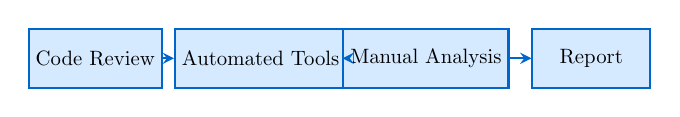
\begin{tikzpicture}[scale=0.75, transform shape, node distance=2.8cm]
\node (code) [process, minimum width=2cm] {Code Review};
\node (auto) [process, right of=code, minimum width=2cm] {Automated Tools};
\node (manual) [process, right of=auto, minimum width=2cm] {Manual Analysis};
\node (report) [process, right of=manual, minimum width=2cm] {Report};

\draw[arrow] (code) -- (auto);
\draw[arrow] (auto) -- (manual);
\draw[arrow] (manual) -- (report);
\end{tikzpicture}
\end{center}

\vspace{3mm}
\textbf{Audit Severity Levels:}
\begin{itemize}
\item \textbf{Critical:} Direct loss of funds---MUST fix before deployment
\item \textbf{High:} Significant risk---should fix
\item \textbf{Medium:} Moderate risk---recommended to fix
\item \textbf{Low:} Minor issues---consider fixing
\item \textbf{Informational:} Suggestions for improvement
\end{itemize}

\vspace{3mm}
\begin{block}{Important Caveat}
Audits are NOT guarantees. Recall from our case studies: the Ronin Bridge (\$625M loss) and Wormhole (\$320M) were both audited. Audits reduce risk but don't eliminate it.
\end{block}
\end{frame}

% =============================================================================
% Frame 32: Bug Bounty Programs
% =============================================================================
%% L5: Added global examples beyond Western platforms
%% H15: Connected bounties to earlier case studies
\begin{frame}{Bug Bounty Programs}
\begin{columns}[T]
\begin{column}{0.55\textwidth}
\textbf{How Bug Bounties Work:}
\begin{itemize}
\item Protocols offer rewards for finding vulnerabilities
\item Ethical hackers report bugs instead of exploiting
\item Rewards scale with severity
\item Continuous security testing
\end{itemize}

\vspace{3mm}
\textbf{Major Platforms (Global):}
\begin{itemize}
\item Immunefi (DeFi-focused, global)
\item HackerOne (global, general-purpose)
\item Code4rena (audit competitions)
\item Slowmist (Asia-Pacific focused)
\item Hacken (Eastern Europe)
\end{itemize}

\vspace{2mm}
\footnotesize \textit{Context:} Had the bZx (\$350K exploit) or Beanstalk (\$182M) protocols offered competitive bounties, ethical hackers might have reported the vulnerabilities first.
\end{column}
\begin{column}{0.42\textwidth}
\textbf{Typical Rewards:}

\vspace{2mm}
\begin{tabular}{lr}
\hline
\textbf{Severity} & \textbf{Reward} \\
\hline
Critical & \$50K--\$10M \\
High & \$10K--\$50K \\
Medium & \$1K--\$10K \\
Low & \$100--\$1K \\
\hline
\end{tabular}

\vspace{5mm}
\begin{alertblock}{Incentive Alignment}
Good bounties make ethical disclosure more profitable than exploitation.
\end{alertblock}
\end{column}
\end{columns}
\end{frame}

% =============================================================================
% Frame 33: Responsible Disclosure
% =============================================================================
%% H15: Connected disclosure to earlier case studies
\begin{frame}{Responsible Disclosure}
\begin{columns}[T]
\begin{column}{0.48\textwidth}
\textbf{Ethical Discovery Process:}
\begin{enumerate}
\item Find vulnerability
\item Document the issue thoroughly
\item Contact protocol team privately
\item Give reasonable time to fix
\item Coordinate public disclosure
\end{enumerate}

\vspace{3mm}
\textbf{DO NOT:}
\begin{itemize}
\item Exploit for personal gain
\item Disclose publicly before fix
\item Demand excessive payment
\item Threaten the protocol
\end{itemize}
\end{column}
\begin{column}{0.48\textwidth}
\textbf{White Hat vs. Black Hat:}

\vspace{3mm}
\textbf{White Hat (ethical):}
\begin{itemize}
\item Reports vulnerabilities
\item Helps fix issues
\item Collects bounty legally
\end{itemize}

\vspace{3mm}
\textbf{Black Hat (malicious):}
\begin{itemize}
\item Exploits for profit
\item Causes financial harm
\item Faces legal consequences
\end{itemize}

\vspace{3mm}
\begin{block}{Gray Area}
Some hackers exploit then return funds (like the Poly Network \$611M case)---legally and ethically ambiguous.
\end{block}
\end{column}
\end{columns}
\end{frame}

% =============================================================================
% Frame 34: Executive Summary
% =============================================================================
\begin{frame}{Executive Summary}
\begin{center}
\textbf{\Large Key Takeaways from Topic 5.1}
\end{center}

\vspace{3mm}
\begin{enumerate}
\item \textbf{Failures fall into three categories:} technical bugs, economic attacks, and human fraud

\item \textbf{Technical exploits} (reentrancy, overflow, access control) can be prevented with secure design patterns

\item \textbf{Economic attacks} (flash loans, oracle manipulation) exploit protocol design assumptions

\item \textbf{Bridges are the biggest target}---69\% of 2022 crypto theft involved bridges

\item \textbf{Defense in depth:} Multiple security layers (CEI, guards, audits, bounties) reduce but don't eliminate risk
\end{enumerate}

\vspace{3mm}
\begin{block}{The Big Idea}
Understanding how things fail is essential for building secure systems. ``Code is law'' only works when the code is correct.
\end{block}
\end{frame}

% =============================================================================
% Frame 35: Concept Map
% =============================================================================
\begin{frame}{Concept Map: Digital Finance Failures}
\begin{center}
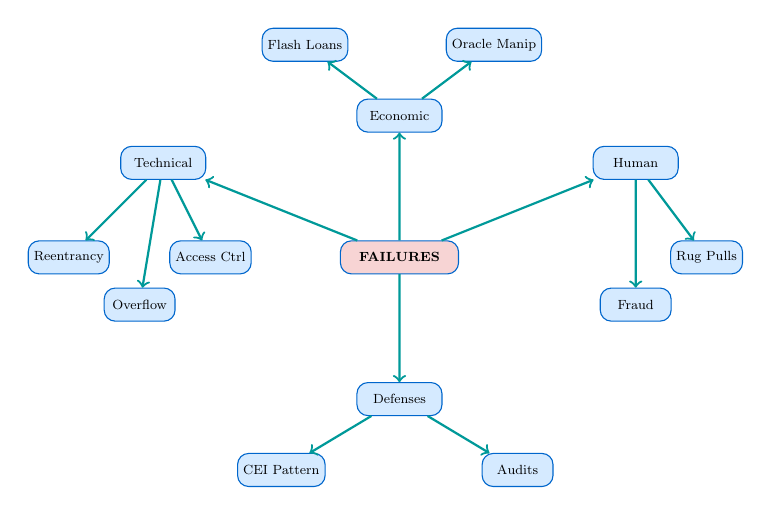
\begin{tikzpicture}[scale=0.6, transform shape,
    concept/.style={rectangle, rounded corners, draw=dfblue, fill=dflightblue4, minimum width=1.8cm, minimum height=0.7cm, font=\footnotesize},
    relationship/.style={->, thick, dfteal}]

% Central concept
\node[concept, fill=dfred!20, minimum width=2.5cm] (failures) at (0,0) {\textbf{FAILURES}};

% Main branches
\node[concept] (technical) at (-5,2) {Technical};
\node[concept] (economic) at (0,3) {Economic};
\node[concept] (human) at (5,2) {Human};
\node[concept] (defense) at (0,-3) {Defenses};

% Technical sub
\node[concept, minimum width=1.5cm] (reentrancy) at (-7,0) {Reentrancy};
\node[concept, minimum width=1.5cm] (overflow) at (-5.5,-1) {Overflow};
\node[concept, minimum width=1.5cm] (access) at (-4,0) {Access Ctrl};

% Economic sub
\node[concept, minimum width=1.5cm] (flash) at (-2,4.5) {Flash Loans};
\node[concept, minimum width=1.5cm] (oracle) at (2,4.5) {Oracle Manip};

% Human sub
\node[concept, minimum width=1.5cm] (rugpull) at (6.5,0) {Rug Pulls};
\node[concept, minimum width=1.5cm] (fraud) at (5,-1) {Fraud};

% Defense sub
\node[concept, minimum width=1.5cm] (cei) at (-2.5,-4.5) {CEI Pattern};
\node[concept, minimum width=1.5cm] (audit) at (2.5,-4.5) {Audits};

% Connections
\draw[relationship] (failures) -- (technical);
\draw[relationship] (failures) -- (economic);
\draw[relationship] (failures) -- (human);
\draw[relationship] (failures) -- (defense);

\draw[relationship] (technical) -- (reentrancy);
\draw[relationship] (technical) -- (overflow);
\draw[relationship] (technical) -- (access);

\draw[relationship] (economic) -- (flash);
\draw[relationship] (economic) -- (oracle);

\draw[relationship] (human) -- (rugpull);
\draw[relationship] (human) -- (fraud);

\draw[relationship] (defense) -- (cei);
\draw[relationship] (defense) -- (audit);
\end{tikzpicture}
\end{center}
\end{frame}

% =============================================================================
% Frame 36: Key Terms & Definitions I
% =============================================================================
\begin{frame}{Key Terms \& Definitions (I)}
\begin{description}
\item[Reentrancy Attack] An exploit where a malicious contract calls back into the victim contract before the first execution completes, allowing repeated withdrawals.

\item[Flash Loan] An uncollateralized loan that must be borrowed and repaid within a single atomic blockchain transaction.

\item[Oracle Manipulation] Artificially moving market prices to deceive protocols that rely on external price data for decision-making.

\item[Check-Effects-Interactions (CEI)] A secure coding pattern: validate conditions (check), update state (effects), then make external calls (interactions).

\item[TWAP] Time-Weighted Average Price---an oracle mechanism that averages prices over time to resist short-term manipulation.
\end{description}
\end{frame}

% =============================================================================
% Frame 37: Key Terms & Definitions II
% =============================================================================
\begin{frame}{Key Terms \& Definitions (II)}
\begin{description}
\item[Rug Pull] A type of fraud where project developers drain funds from a liquidity pool or abandon a project after collecting investments.

\item[Bridge Exploit] An attack targeting cross-chain bridges, which hold large amounts of locked assets and have complex security surfaces.

\item[Defense in Depth] A security strategy using multiple independent layers of protection, so failure of one layer doesn't compromise the system.

\item[Bug Bounty] A program offering rewards to ethical hackers who discover and responsibly disclose security vulnerabilities.

\item[Systemic Risk] The risk that failure of one protocol cascades through interconnected systems, affecting the entire ecosystem.
\end{description}
\end{frame}

% =============================================================================
% Frame 38: Common Misconceptions
% =============================================================================
\begin{frame}{Common Misconceptions}
\begin{columns}[T]
\begin{column}{0.48\textwidth}
\textbf{\textcolor{dfred}{Misconception}}

\vspace{2mm}
``Audited means safe''

\vspace{5mm}
``DeFi eliminates all trust''

\vspace{5mm}
``Smart contracts are always correct''

\vspace{5mm}
``Flash loans are inherently malicious''
\end{column}
\begin{column}{0.48\textwidth}
\textbf{\textcolor{dfgreen}{Reality}}

\vspace{2mm}
Many exploited protocols had multiple audits; audits reduce but don't eliminate risk

\vspace{2mm}
Trust shifts from institutions to code, oracles, and governance---different trust, not zero trust

\vspace{2mm}
Code can have bugs, logic errors, and unforeseen interactions just like any software

\vspace{2mm}
Flash loans have many legitimate uses (arbitrage, collateral swaps); they're tools that can be misused
\end{column}
\end{columns}

\vspace{5mm}
\begin{alertblock}{Critical Thinking}
Always ask: What are the assumptions? What happens if they're wrong? Who holds the keys?
\end{alertblock}
\end{frame}

% =============================================================================
% Frame 39: Self-Assessment Question 1
% =============================================================================
%% M10: Added conceptual question alongside technical one
\begin{frame}{Self-Assessment: Question 1}
\begin{block}{Question}
A bank teller hands you cash and THEN checks your account balance. If you keep asking for cash before the teller finishes checking, what type of smart contract attack does this resemble?
\end{block}

\vspace{3mm}
\begin{enumerate}[A.]
\item A flash loan attack
\item A reentrancy attack
\item An oracle manipulation
\item A rug pull
\end{enumerate}

\vspace{5mm}
\pause
\textbf{Answer: B}

\vspace{2mm}
\textbf{Explanation:} A reentrancy attack occurs when a contract sends money (like the teller handing out cash) before updating its records. The attacker exploits this gap by requesting money again before the records are updated, draining the contract repeatedly.
\end{frame}

% =============================================================================
% Frame 40: Self-Assessment Questions 2-3
% =============================================================================
%% M10: Added conceptual question (Q2 rewritten for non-technical audience)
\begin{frame}{Self-Assessment: Questions 2--3}
\begin{block}{Question 2}
Why are flash loans especially dangerous, even though the attacker has to return the money?
\end{block}
\textbf{Answer:} Because the attacker can temporarily control enormous amounts of capital (millions of dollars) to manipulate prices or exploit vulnerabilities, and if the attack fails, they lose nothing---the transaction simply reverses. The risk is entirely one-sided.

\vspace{5mm}
\begin{block}{Question 3}
A restaurant where the waiter brings food to every table (push) vs. a buffet where guests serve themselves (pull)---which is safer for smart contracts and why?
\end{block}
\textbf{Answer:} The pull (buffet) pattern is safer. In the push pattern, one problematic recipient can block payments to everyone else. In the pull pattern, each user withdraws independently, so one failure doesn't affect others. This also reduces reentrancy risk.
\end{frame}

% =============================================================================
% Frame 41: What's Next - Preview T5.2
% =============================================================================
\begin{frame}{What's Next: Topic 5.2}
\begin{center}
\textbf{\Large Preview: Regulatory Landscapes}
\end{center}

\vspace{5mm}
\textbf{In Topic 5.2, we'll explore:}
\begin{itemize}
\item How \textbf{governments respond} to digital finance failures
\item Comparison of \textbf{regulatory frameworks} (US, EU, Asia)
\item The \textbf{securities law} question: When is a token a security?
\item \textbf{AML/KYC requirements} and their implications
\item Emerging \textbf{stablecoin regulations}
\end{itemize}

\vspace{5mm}
\begin{block}{Connection}
Topic 5.1 examined \textit{what goes wrong} technically and economically.\\
Topic 5.2 examines \textit{how regulators respond} to these failures.
\end{block}

\vspace{3mm}
\textbf{Preparation:} Consider how the failures we discussed today might influence regulatory approaches.
\end{frame}

% =============================================================================
% Frame 42: Resources
% =============================================================================
\begin{frame}{Resources for Further Learning}
\textbf{Essential Reading:}
\begin{itemize}
\item Rekt News (\url{rekt.news})---detailed post-mortems of DeFi exploits
\item ``Smart Contract Security Best Practices'' (ConsenSys Diligence)
\item Chainalysis Crypto Crime Reports (annual)
\end{itemize}

\vspace{3mm}
\textbf{Online Resources:}
\begin{itemize}
\item Course notebook: \texttt{NB11\_DeFi\_Exploits.ipynb}
\item DeFiLlama Hacks Dashboard (\url{defillama.com/hacks})
\item Immunefi Bug Bounty Platform (\url{immunefi.com})
\end{itemize}

\vspace{3mm}
\textbf{Technical Deep Dives:}
\begin{itemize}
\item SWC Registry (Smart Contract Weakness Classification)
\item OpenZeppelin Security Blog
\item Samczsun's Blog (security researcher)
\end{itemize}

\vspace{3mm}
\begin{block}{Course Materials}
All slides and notebooks available on the course website.
\end{block}
\end{frame}

% =============================================================================
% Frame 43: Questions?
% =============================================================================
\begin{frame}{Questions?}
\begin{center}
\textbf{\LARGE Questions \& Discussion}

\vspace{10mm}
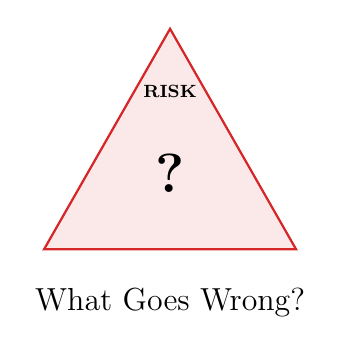
\begin{tikzpicture}[scale=0.8, transform shape]
% Warning sign with question
\draw[thick, dfred, fill=dfred!10] (0,0) -- (2,3.5) -- (4,0) -- cycle;
\node at (2,1.2) {\Huge \textbf{?}};
\node at (2,2.5) {\footnotesize \textbf{RISK}};
\node[below] at (2,-0.5) {\Large What Goes Wrong?};
\end{tikzpicture}

\vspace{10mm}
\textbf{Contact:} joerg.osterrieder@ifi.uzh.ch

\vspace{3mm}
\textbf{Next Topic:} T5.2 --- Regulatory Landscapes
\end{center}
\end{frame}

\end{document}
